\documentclass{beamer}
\usepackage[utf8]{inputenc}
\usepackage[spanish]{babel}
\usepackage{graphicx}
\usepackage{booktabs}
\usepackage{ragged2e}
\usepackage{xcolor}
\definecolor{LightGray}{gray}{0.975}
\definecolor{links}{HTML}{2A1B81}
%\usepackage[urlcolor=blue]{hyperref}
\hypersetup{colorlinks,linkcolor=,urlcolor=blue}

\usepackage{tikz}
\usetikzlibrary{arrows,shapes}

\usepackage{algorithm}
\usepackage{algorithmic}

\usepackage{minted}
\usepackage{xcolor}
\definecolor{LightGray}{gray}{0.975}

\usepackage{listings}

%\usetheme{Warsaw}
\usefonttheme{serif} 

\title[Monitoring]{Database Administration}
\subtitle{Lecture 05: Performance Monitoring and Tuning.}
\author{Ciolli et al. and Grafana Labs.}
\date{\today}

\setbeamertemplate{navigation symbols}{}%remove navigation symbols

\defbeamertemplate*{footline}{shadow theme}
{%
  \leavevmode%
  \hbox{\begin{beamercolorbox}[wd=.5\paperwidth,ht=2.5ex,dp=1.125ex,leftskip=.3cm plus1fil,rightskip=.3cm]{author in head/foot}%
    \usebeamerfont{author in head/foot} Database Administration \hfill \insertshorttitle
  \end{beamercolorbox}%
  \begin{beamercolorbox}[wd=.5\paperwidth,ht=2.5ex,dp=1.125ex,leftskip=.3cm,rightskip=.3cm plus1fil]{title in head/foot}%
    \usebeamerfont{title in head/foot} \hfill \insertframenumber\,/\,\inserttotalframenumber%
  \end{beamercolorbox}}%
  \vskip0pt%
}

\AtBeginSection[]
{
     \begin{frame}<beamer>
     \frametitle{Plan}
     \tableofcontents[currentsection]
     \end{frame}
}

\newcommand{\toRight}[1]{
    \begin{FlushRight}
        {\tiny #1}
    \end{FlushRight}
} % Align to right

\begin{document}

\frame{\titlepage}

\begin{frame}{Database Administration: Reverse Design.}
    \centering
    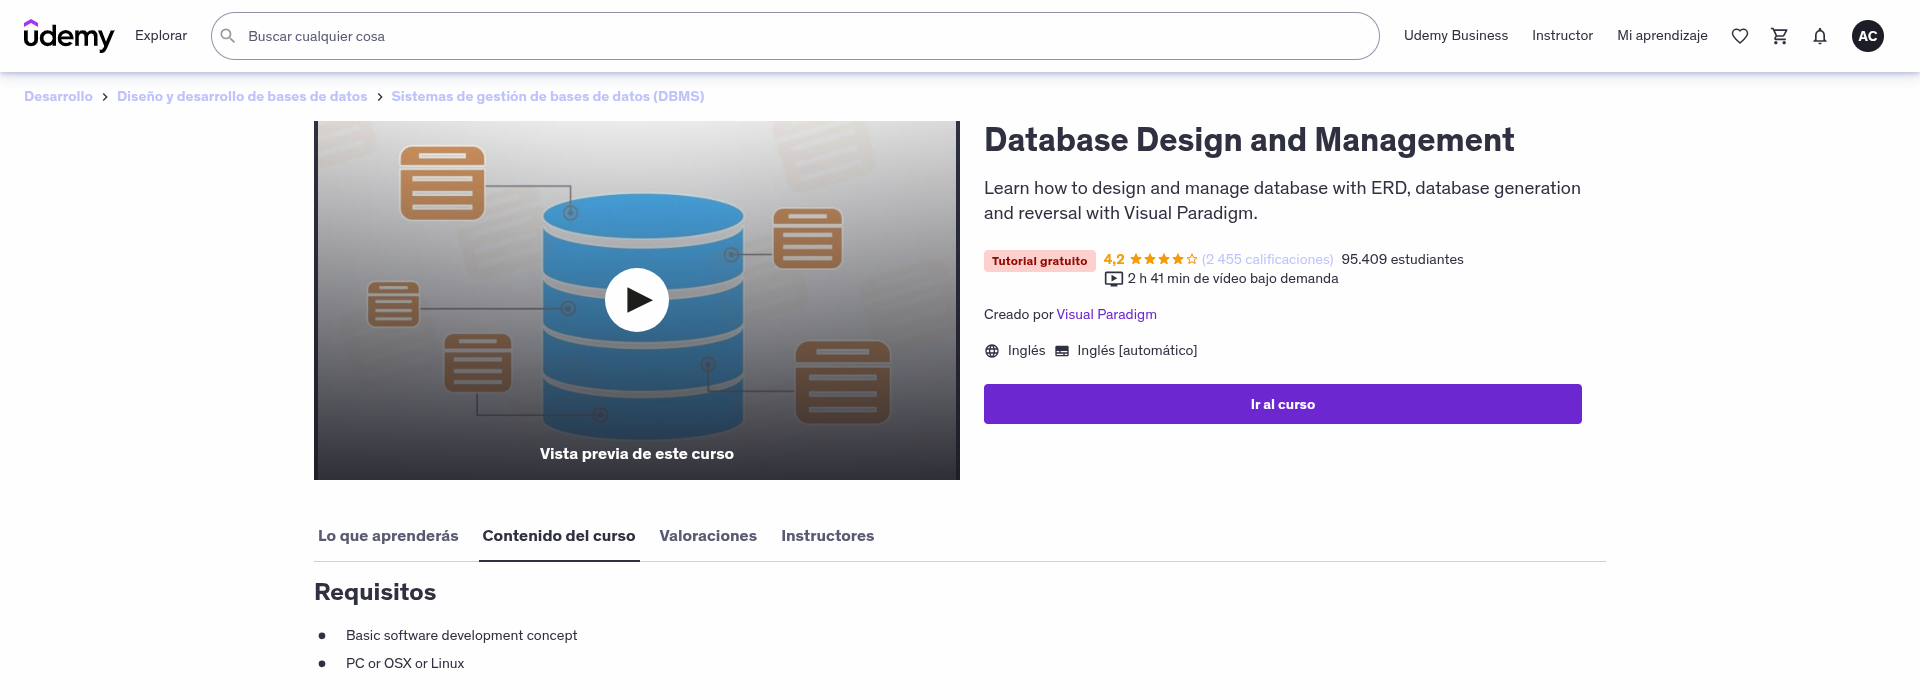
\includegraphics[width=\textwidth]{figures/udemy2}\\
    
\includegraphics[width=\textwidth]{figures/udemy3}\\
    \vspace{2mm}
    {
        \scriptsize
        Content has been extracted from \textit{Database Design and Management.} Udemy Course, created by Visual Paradigm, 2025.  Visit \url{https://www.udemy.com/course/database-design-and-management/} and \url{https://www.visual-paradigm.com/}.\\
    }
\end{frame}


\begin{frame}{}
    \centering
    \Huge End of Lecture 4.
\end{frame}

\section*{Takeaways}

% Tim Duncan's Top 5 Fundamental Takeaways of the Today's Class
\begin{frame}{TDT5FTOTTC}
    \centering
    
\includegraphics[width=0.75\textwidth]{figures/tim.png}
\end{frame}

\begin{frame}{Top 5 Fundamental Takeaways}
    \small
    \begin{enumerate} \pause
        \item[5] \textbf{Database Views, Triggers, and Stored Procedures} enhance database security, automation, and efficiency by providing pre-queried data, event-based actions, and reusable SQL routines. \pause

        \item[4] \textbf{Keys and Relationships} define how data is uniquely identified (Primary Keys), linked across tables (Foreign Keys), and structured using Composite Keys for complex relationships. \pause

        \item[3] \textbf{Normalization} and Database Optimization help minimize data redundancy and balance between normalized (integrity-focused) and denormalized (performance-oriented) structures. \pause

        \item[2] \textbf{Three Levels of ER Modeling} include the conceptual (high-level overview), logical (detailed structure with normalization), and physical (implementation-specific design). \pause

        \item[1] \textbf{ERDs (Entity-Relationship Diagrams)} provide a visual representation of database structures and relationships to improve data organization and communication. \pause
        \end{enumerate}
\end{frame}


\begin{frame}{Database Administration: Reverse Design.}
    \centering
    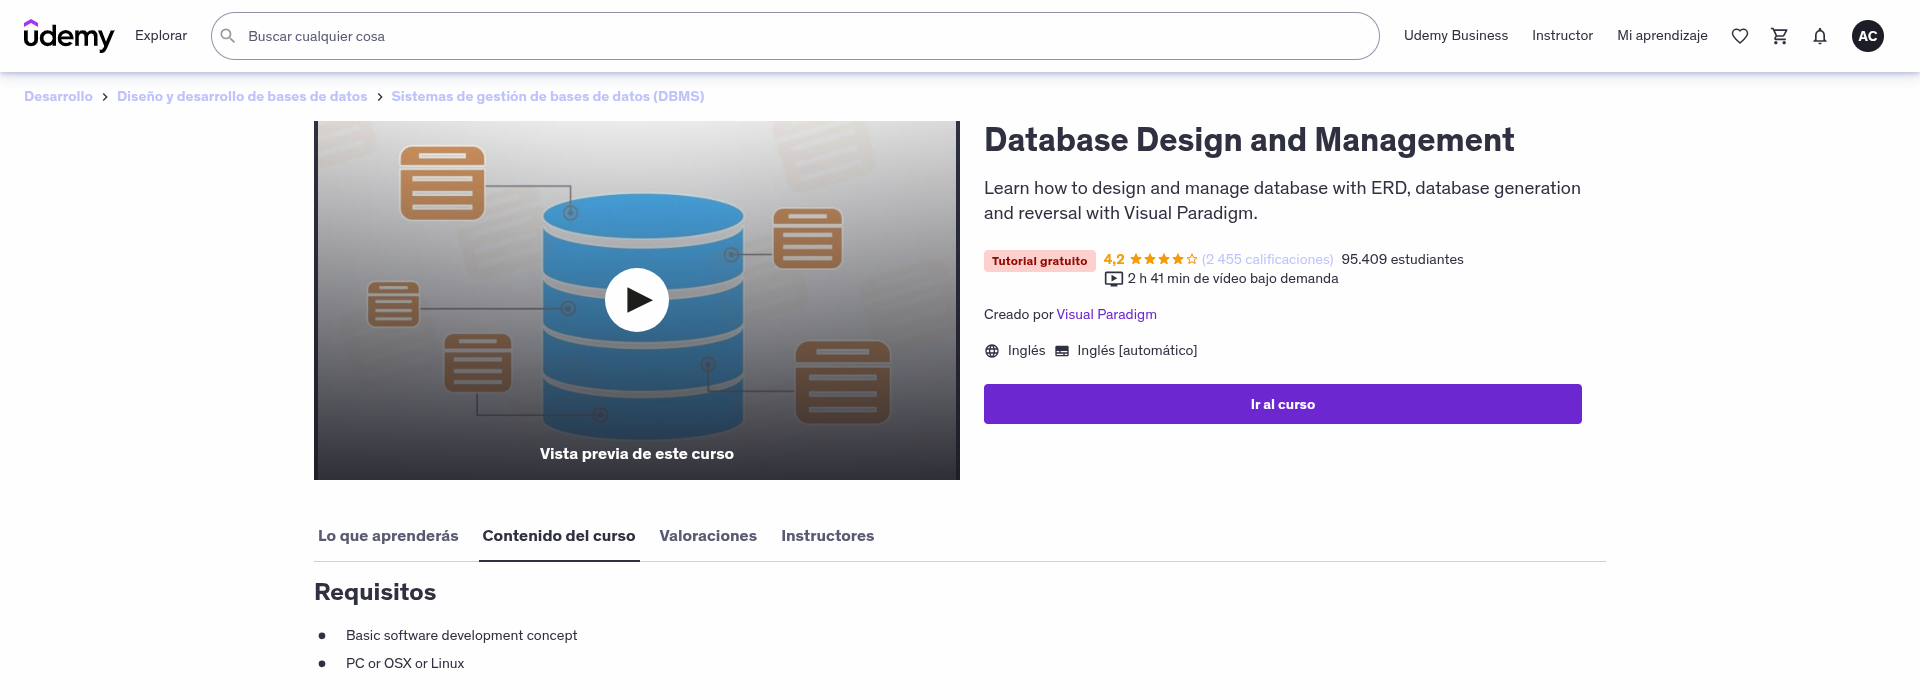
\includegraphics[width=\textwidth]{figures/udemy2}\\
    
\includegraphics[width=\textwidth]{figures/udemy3}\\
    \vspace{2mm}
    {
        \scriptsize
        Content has been extracted from \textit{Database Design and Management.} Udemy Course, created by Visual Paradigm, 2025.  Visit \url{https://www.udemy.com/course/database-design-and-management/} and \url{https://www.visual-paradigm.com/}.\\
    }
\end{frame}

\end{document}
